\chapter{Research Contribution}
% \textbf{***focus on dp federated while we allow some public useres}
The main goal of the research is to use some small number of \textit{public users} - paid users who consented to their private data being exposed - to express gradients during the federated learning process. Applying differential privacy mechanism to the estimated gradients will enable better privacy budget using less noise and thus better learning.
\section{Differentially Private Federated Learning  Setup for EMG Data }
EMG data is naturally acquired in a federated manner by sensing the different users using wrist bands. The internal epoch done locally on users device are considered private. This means that no matter how many times the local model "sees" the private data, the gradients are then sent to the aggregator are considered as a single data sample contribution. Moreover, several "paid" users agreed to make their data not differntially private. This public subset enables the use of methods like GEP \cite{Yu2021DoLearning} 
\subsection{Federated GEP}
In the federated GEP setup we mark some users as "public" and use them to create the gradient anchor subspace. 

At each learning iteration:
\begin{itemize}
    \item Users get the updated model weights from the aggregator
    \item Every user perform internal train for some predefined number of epochs
    \item Users return the internal train gradients to the aggregator
\end{itemize}
 The above learning process is repeated till convergence. No data is transferred outside users' device/computer. The only sensitive part are the transferred gradients. These gradients reflect knowledge about users' data and needed to be differentially private.
 \subsubsection{Internal Local Train}
 All data is present on users' device, hence the feed forward, loss and gradients computation is done locally on each users' device.
 The internal train is considered private without the need to perturb the gradients between epochs. The resulting gradients are the difference between the baseline model and the trained model after internal train. The aggregator receives a "batch" of user gradients - each user is a sample. The gradients are then projected to the public anchor subspace. By definition, the resulting embedded gradients are the best approximation of the original gradients in the anchor subspace. In order to reconstruct the original gradient from the embedded one, a \textit{residual} gradient needs to be added. To achieve differential privacy, the embedded gradients and the residual gradients are perturbed separately and then averaged and back-propagated in the global model.

Some more training details:
\begin{itemize}
    \item Start with pretrained model - trained on public users
    \item Freeze local train learning rate during internal epochs or just subtract the weights at the beginning of the local train from the current ones
    \item Adjust the global model learning rate accordingly
\end{itemize}


% \section{Toy Story Dataset and Users}
% For ease and flexibility of training and parameter change a toy problem (TOY STORY) is used.

% TOY STORY is a federated learning regression problem defined as follows:
% \begin{itemize}
%     \item Users have IDs ['001', '002', ...,'170', ...] and are splitted to TRAIN USERS, VALIDATION USERS and TEST USERS. The total amount and splits are configured.
%     \item Public Users are some subset of TRAIN USERS
%     \item The data are numbers or arrays randomly generated and the labels are the result of the polynomial with DATA\_COEFFS coefficients and the input data substituted. The data inputs scale and dimension are configured
%     \item Each user has a typical Bias\\Variance features that controls how he labels the data. 
% \end{itemize}

% The federated training is done as follows:
% \begin{itemize}
%     \item At global epoch start, some users are sampled according to configured amount. This will control the 'q' (sampling probability) variable in the accountant
%     \item Each sampled user gets new generated data and the current model weights. Data size for each internal epoch is configured. 
%     \item User performs train epoch for the received data. The labels are noised by the user's bias and variance. (Note that this noise is not DP related,  It's just the user personal features). At the end of this internal epoch, the user returns its gradients to the aggregator. Till now no DP is done.
%     \item The aggregator gets all users gradients, preforms the clipping and noising according to the tested algorithm. Note that in the aggregator context, the batch size is the number of aggregated users and internal gradients are a single sample.
    
% \end{itemize}
 
\section{Research Directions}
\begin{itemize}

    \item \textbf{Backbone for putEMG} - Several alternative architectures to learn putEMG data were tested. Mainly focused on convolution models and specifically 3D convolution to capture the two dimensions of the wrist band and the time dimension. Some more potential architectures to be may include transformers or other attention modules.

    \item \textbf{Median of Signs} -  Compute sign of per-sample gradient and take the median of signs. Unless \\ $\#\{ \textit{positive gradients}\} - 1 \leq \#\{\textit{negative gradients}\} \leq \#\{\textit{positive gradients}\} + 1 $, this method is not sensitive to a single sample. For sensitive iterations skip backpropagation and zero grad. No noise is needed because privacy is achieved by median.

    \item \textbf{Sample Gradient Distribution} - Estimate Gradient distribution by mean and standard deviation of batch direction at each dimension. Sample from this distribution and use the sample for backpropagation. Another alternative is learn the gradients distribution using a GP.

    \item \textbf{Gradient Embedding Perturbation} - Use a GEP variant
    by :
    \begin{itemize}
        \item Compute low rank subspace by PCA instead of power method
        \item Aggregate past gradients in order to span a better subspace using few public users
    \end{itemize}

    % \item \textbf{Do not perturb local federated trains gradients}

    % \item  \textbf{Measure Accuracy-Privacy Hints} - 
    % \begin{itemize}
    %     \item Max Probability value of predictions
    %     \item Train-Test per label distance (KL divergence)
    %     \item Ability to reconstruct train set (Niv Haim from Weizman)
    % \end{itemize}  

    \item \textbf{Apply \textit{Deepmind}'s technical report \cite{DeUnlockingScale} methods}
    

     Take a full GD for a toy problem and look at gradient vector field
    
\end{itemize}

\section{Initial Experimental Results}
Initial experimental runs  were done to compare the privacy and performance achieved using GEP with and without residuals compared to DP-SGD.

 \begin{itemize}
           \item Experiments were done on CIFAR10 datset
           \item Learned using a simple MLP model
           \item 500 train users, each know 2 classes out of 10.
           \item 4 paid users are considered public users. Their learning process is used to span the subspace all gradients are projected to.
 \end{itemize}
  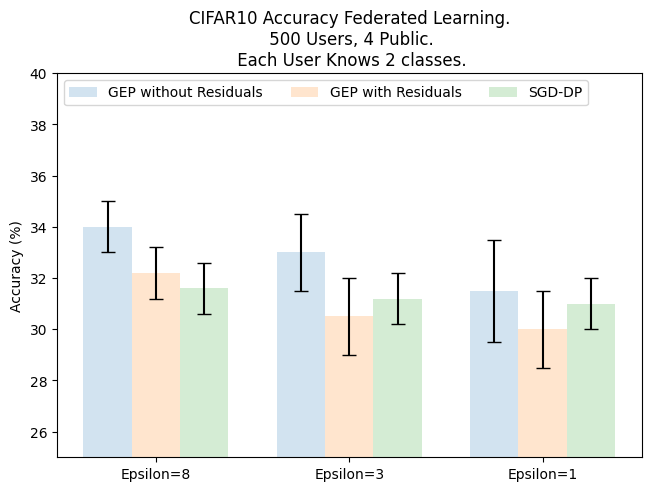
\includegraphics[height = 0.55\textwidth]{images/cifar10_dpsgd_vs_gep.png} \\
  From the initial results we see that if the privacy budget is $ \geq 3$, the advantage looks clear, but if it is low, the advantage is not so apparent. We hope to achieve better performance even for smaller privacy budget.